\documentclass[11pt,a4paper]{article}

\usepackage[T1]{fontenc}
\usepackage[utf8]{inputenc}
\usepackage{lmodern}
\usepackage{microtype}
\usepackage[margin=2.3cm]{geometry}
\usepackage{amsmath}
\usepackage{booktabs}
\usepackage{array}
\usepackage{tabularx}
\usepackage{longtable}
\usepackage{enumitem}
\usepackage{xcolor}
\usepackage{rotating}
\usepackage{float}
\usepackage{pgfplots}
\usepgfplotslibrary{groupplots}
\pgfplotsset{compat=1.18}
\usepackage{hyperref}

\definecolor{workinggreen}{HTML}{1B7F3A}
\definecolor{wiporange}{HTML}{A85D00}
\definecolor{pendingred}{HTML}{A32121}
\definecolor{linkblue}{HTML}{1E5A96}

\hypersetup{
  colorlinks=true,
  linkcolor=linkblue,
  urlcolor=linkblue,
  citecolor=linkblue,
  pdftitle={LM-IDNet Full Project Report}
}

\setlength{\parindent}{0pt}
\setlength{\parskip}{0.65em}
\setlist[itemize]{topsep=0.25em,itemsep=0.2em,leftmargin=1.6em}
\setlist[enumerate]{topsep=0.25em,itemsep=0.2em,leftmargin=1.8em}
\renewcommand{\arraystretch}{1.2}

\newcommand{\projectname}{LM-IDNet}
\newcommand{\working}{\textcolor{workinggreen}{\textbf{Working on master}}}
\newcommand{\wip}{\textcolor{wiporange}{\textbf{Experimental/WIP}}}
\newcommand{\notdone}{\textcolor{pendingred}{\textbf{Not completed}}}

\title{\textbf{LM-IDNet Full Project Report}\\
\large Working System, Experimental Evidence, and Ongoing Research}
\author{Prepared for supervisor review}
\date{9 September 2026}

\begin{document}

\maketitle
\thispagestyle{empty}

\begin{abstract}
This report presents the complete current state of \projectname{}, a lightweight,
unsupervised anomaly detector for Internet of Things network traffic. The
working system on the \texttt{master} branch converts packet captures into
ten-minute traffic-count windows, fits a Dirichlet--multinomial normal model,
calibrates an anomaly threshold, emits interpretable decisions, evaluates
labelled development traffic, and supports both threshold adaptation and
guarded periodic model refitting. The specialised Languasco--Migliardi numerical
method has been integrated as a safe native likelihood backend and compared
directly with SciPy. The report also documents two separate research tracks: one
checks the true time ordering of the data, and the other tests additional traffic
measurements. Their useful findings are included, but they are not presented as
features of the reference branch. The result is an account of what was built,
what was measured, what failed, and what remains before a final thesis claim can
be made.
\end{abstract}

\vfill
\begin{center}
\begin{minipage}{0.90\textwidth}
\small
\textbf{Versions covered.} The reference implementation in this report is
\texttt{master} at commit \texttt{cb8dd66}. Temporal-fold work is read from
\texttt{feature/temporal-model} at \texttt{b0aa35d}; the wider detector study is
read from \texttt{feature/volume-anomaly} at \texttt{4279d84}. Detection results
and branch findings are taken from committed JSON artefacts and experiment
records; the three-dataset timing comparison was rerun for this report. A branch
result is labelled as such wherever it appears, so working software, development
evidence, and future work remain distinct.
\end{minipage}
\end{center}

\newpage
\tableofcontents
\newpage

\section{Executive Summary}

\subsection{What the project is}

\projectname{} learns the ordinary network behaviour of one IoT device without
using attack examples during training. Traffic is reduced to counts of TCP,
ordinary UDP, SSDP, and ARP packets in consecutive ten-minute windows. A
Dirichlet--multinomial model describes the expected mixture and its normal
variation. Later windows receive a log-probability score; an independently
calibrated lower-tail threshold turns that score into an anomaly decision.

The implementation is a reproducible command-line research system rather than
one large script. Each stage reads declared inputs and writes inspectable JSON.
The central path is:

\begin{center}
\fbox{\begin{minipage}{0.94\textwidth}
\centering
packet captures $\longrightarrow$ validated device windows
$\longrightarrow$ normal model $\longrightarrow$ benign calibration\\[0.35em]
$\longrightarrow$ static or adaptive scoring
$\longrightarrow$ labelled evaluation and audit reports
\end{minipage}}
\end{center}

\subsection{Current project position}

The reference branch contains a complete offline detector: it validates and
processes packet captures, fits and calibrates a normal model, scores later
traffic, explains each decision, and evaluates labelled development data. The
stored results show high precision but incomplete recall, while the numerical
benchmarks show that the native LM backend agrees closely with SciPy. Adaptation
is one completed experimental stage within this larger system; its strongest
configuration is still a development candidate rather than a final result.

\begin{table}[H]
\centering
\small
\begin{tabularx}{\textwidth}{>{\raggedright\arraybackslash}p{0.25\textwidth}
>{\raggedright\arraybackslash}p{0.21\textwidth} X}
\toprule
\textbf{Area} & \textbf{Status} & \textbf{Evidence available now} \\
\midrule
Reference detector & \working & PCAP preprocessing, fitting, calibration,
development scoring, explanations, and labelled evaluation for two devices. \\
Numerical method & \working & Native LM integration, SciPy comparison, stress
tests, and benchmarks of both the production detector and the paper-style
experiment. \\
Adaptation & \working & Static, threshold-only, and guarded periodic-refit modes
with isolated configurations, events, evaluations, and update audits. \\
Temporal evaluation & \wip & A separate branch checks actual timestamps and
overlaps, evaluates several chronological splits, and reports results by capture
and attack episode. \\
Multi-signal detector & \wip & A separate experiment branch tests traffic
volume, direction, connection behaviour, and ARP activity, and measures scoring
cost. \\
Final thesis evaluation & \notdone & The current master detector and its tuned
adaptive policy have not been tested on a predeclared, untouched final set. \\
Production edge deployment & \notdone & Development-host measurements exist in
the experiment branch, but no target edge device has been benchmarked. \\
\bottomrule
\end{tabularx}
\caption{Status of the project at the time of this report.}
\label{tab:executive-status}
\end{table}

\begin{figure}[H]
\centering
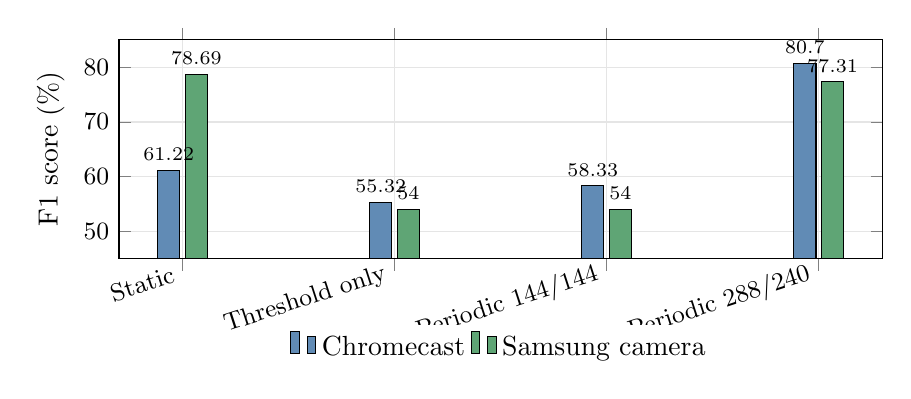
\begin{tikzpicture}
\begin{axis}[
  ybar,
  bar width=8pt,
  width=0.93\textwidth,
  height=0.36\textwidth,
  ymin=45,
  ymax=85,
  ylabel={F1 score (\%)},
  symbolic x coords={static,threshold,periodic144,periodic288},
  xtick=data,
  xticklabels={Static,Threshold only,Periodic 144/144,Periodic 288/240},
  x tick label style={font=\small,rotate=18,anchor=east},
  y tick label style={font=\small},
  grid=major,
  grid style={gray!20},
  legend style={draw=none,at={(0.5,-0.30)},anchor=north,legend columns=2},
  nodes near coords,
  nodes near coords style={font=\scriptsize},
]
\addplot[fill=linkblue!70] coordinates {
  (static,61.22) (threshold,55.32) (periodic144,58.33) (periodic288,80.70)
};
\addlegendentry{Chromecast}
\addplot[fill=workinggreen!70] coordinates {
  (static,78.69) (threshold,54.00) (periodic144,54.00) (periodic288,77.31)
};
\addlegendentry{Samsung camera}
\end{axis}
\end{tikzpicture}
\caption{Master-branch development comparison. The 288/240 result is selected
development evidence, not a locked final result.}
\label{fig:headline-f1}
\end{figure}

\subsection{What has been learned}

The project has established a reproducible path from packet captures to
auditable anomaly decisions, and it has shown where that path is strong and
where it is still limited. The four protocol counts provide a compact and
interpretable baseline, but protocol proportions alone miss attacks that mainly
change traffic volume, direction, or connection behaviour. The native LM
implementation agrees with SciPy and is fast enough for online scoring, although
its speed advantage depends on the operation and dataset. Chronological capture
splits are safer than random window splits, but several time boundaries and
episode-level results are needed before a general detection claim can be made.
Finally, adaptation can improve recall, but it can also learn from attacks if its
safety checks are too weak. These findings make the remaining work clear:
consolidate the temporal safeguards, compare the baseline with the smallest
supported set of additional signals, improve adaptation safety, and then freeze
the complete detector for final evaluation.

\section{Research Problem and Scientific Basis}

\subsection{Why IoT traffic can be modelled as counts}

Many IoT devices perform a narrow set of tasks and repeatedly communicate with
the same local and cloud services. Their traffic is not constant, but its protocol
mixture often has a recognisable structure. For one window the system stores

\[
\mathbf{x}=(x_{\mathrm{TCP}},x_{\mathrm{UDP}},x_{\mathrm{SSDP}},x_{\mathrm{ARP}}),
\qquad N=\sum_k x_k.
\]

The categories are mutually exclusive: SSDP is separated from the remaining UDP
traffic. This representation is small enough for an edge-oriented detector and
retains protocol-level evidence that can be explained to an operator.

A fixed multinomial distribution is often too rigid because ordinary device
behaviour changes from window to window. The Dirichlet--multinomial distribution
adds this overdispersion through a positive parameter vector
$\boldsymbol{\alpha}$. Its expected traffic mixture is
$\alpha_k/\alpha_0$, where $\alpha_0=\sum_k\alpha_k$. The project also reports
$\psi=1/\alpha_0$ as a compact dispersion indicator.

The complete log-probability of a window is

\[
\log P(\mathbf{x}\mid\boldsymbol{\alpha})
=\log\frac{N!}{\prod_k x_k!}
+\log\frac{\Gamma(\alpha_0)}{\Gamma(\alpha_0+N)}
+\sum_k\log\frac{\Gamma(\alpha_k+x_k)}{\Gamma(\alpha_k)}.
\]

A low score means that the observed mixture is unlikely under the normal model.
The decision threshold $\tau$ is learned from a separate benign calibration
period:

\[
\text{anomaly if }\log P(\mathbf{x}\mid\boldsymbol{\alpha})<\tau.
\]

The versioned experiments use a raw score and a one-percent lower calibration
quantile. Per-packet normalisation remains available as a separate experiment;
it is not silently mixed with the reported results.

\subsection{The role of the LM method}

The Languasco--Migliardi (LM) method evaluates close log-Gamma differences
accurately inside the Dirichlet--multinomial likelihood \cite{lmcore,tpami}.
Parameter estimation uses Minka's
fixed-point equations \cite{minka}; LM or SciPy supplies the likelihood used for
convergence checks and scoring.

This distinction prevents an important overclaim. A numerical backend can change
runtime and numerical behaviour near the multinomial limit, but it does not make
an unchanged statistical detector inherently more accurate. The system keeps a
SciPy implementation as an independent reference and selects six-digit native LM
in the versioned research configurations.

\subsection{Relation to the supplied IoT work}

The reference study models D-Link Camera 5 traffic as daily ten-minute vectors
with the same four categories and compares likelihood methods in modelling and
forecasting experiments \cite{iotpaper}. \projectname{} retains that statistical
foundation but changes the application protocol. It fits one device baseline,
uses a separate threshold-calibration period, emits anomaly decisions, and tests
those decisions on labelled traffic from additional IoT devices.

The D-Link captures remain useful as a matched numerical workload. They do not
contain attack labels in this repository, so they cannot support measured
precision, recall, or F1. This is why the main anomaly results use UNSW Chromecast
and Samsung camera traces instead.

\section{Implementation Work Completed on the Master Branch}

\subsection{Foundation, configuration, and operational controls}

The early scaffold was converted into an installable Python package with a
neutral Docker entry point and one authoritative dependency file. Its command
line separates preprocessing, modelling, calibration, scoring, adaptation,
evaluation, and benchmarking into explicit stages. Commands return structured
output, use stable error codes, support non-mutating dry runs, and write UTC
logs.

Each device has a strict JSON configuration. It records the device identity and
MAC address, input and output locations, protocol order, window length,
chronological partitions, estimator, likelihood backend, calibration rule,
adaptation mode, and random seeds. Misspelled fields, inconsistent category
counts, invalid quantiles, duplicate capture assignments, reversed partitions,
and impossible adaptation buffer sizes are rejected before a run begins. The
shell experiment runner selects reviewed configuration files instead of
requiring detector edits for each run.

Pydantic schemas validate models, thresholds, events, and manifests when they
are loaded. Model and dataset fingerprints also prevent artefacts from different
runs from being combined merely because their filenames look compatible.

\subsection{Data engineering and capture validation}

Source PCAPs can first be inventoried, read completely for structural validation,
or fingerprinted without running model code. The fingerprint hashes both capture
bytes and the policies that give those bytes meaning, including category order,
windowing, and partition assignment. A changed file or experiment definition
therefore produces a different dataset identity.

The processor selects one device by Ethernet or ARP hardware address. It filters
raw frames before asking Scapy to decode them, an important improvement for large
mixed-device captures. An experiment on a 1.48~GB UNSW capture recorded a
reduction from 280.0 seconds to 12.5 seconds with byte-identical processed JSON.

Retained packets are classified once, timestamps are normalised to UTC, and
counts are placed in epoch-aligned half-open intervals $[t,t+10\text{ minutes})$.
Observed silence is stored as a valid zero vector. Missing capture coverage is a
different state and is excluded from model fitting and scoring. This distinction
prevents ``the device sent nothing'' from being confused with ``the recording
contains no evidence.''

The Chromecast and Samsung captures were filtered and converted into this common
window format. Their official attack annotations were stored separately using
the same capture ID and exact time bounds as the scored windows. Provenance
records document retained and excluded captures, incomplete days, file hashes,
attack intervals, and partition choices.

\subsection{Statistical modelling, calibration, and scoring}

Training loads only the declared fit captures, checks the device and category
names, and fits $\boldsymbol{\alpha}$ with Minka's fixed-point estimator. The
saved model identifies the source data, capture IDs, number of windows, and UTC
range. It also records the numerical backend, precision, fitted parameters,
whether fitting converged, the iteration count, the likelihood, and the runtime.

Calibration then scores a different benign partition. It stores the chosen
quantile, threshold, score distribution, and interquartile range. The threshold
also carries a deterministic model fingerprint. A model change invalidates the
old threshold rather than allowing an apparently compatible filename to pass.

Static scoring keeps the fitted model and threshold fixed. Every non-missing
development window produces an event containing its counts, score, decision,
severity, expected profile, category residuals, and model fingerprint. Residuals
identify which categories were high or low relative to expectation. They are a
local explanation, not an attack-family diagnosis.

The same pipeline also produces descriptive count statistics and separate daily
Dirichlet fits. Raw and per-packet-normalised score conventions are available as
explicit alternatives, but the reported detector uses raw scores throughout.
Because every event identifies its source data, model, and threshold, detector
variants can be compared window by window without guessing which artefacts were
used.

\subsection{Labelled evaluation}

Attack labels are stored separately from processed counts. Evaluation joins a
decision and label only when capture ID and exact time bounds agree. Duplicate
matches are rejected, and unmatched counts are reported. The evaluator produces
the confusion matrix, accuracy, precision, recall, and F1. Labels are never
loaded during training, calibration, or adaptive updates.

The current \texttt{master} evaluator is deliberately limited to the development
partition. Final capture IDs exist in configuration, but the reference scoring
path has not yet been opened for a locked final run.

\subsection{Native LM integration}
\label{sec:lm-changes}

The professor-supplied code under \path{lm-algorithm/code/} is preserved as a
reference. The application calls a separate production copy under
\path{src/lm_idnet/algorithms/native/}. The mathematical approximation is
unchanged; the integration work makes it safe and efficient to use inside the
detector:

\begin{enumerate}
  \item Zero counts return the exact zero log-Gamma difference, so sparse and
  fully silent windows are valid inputs.
  \item Coefficient paths, file reads, and allocations are checked, and native
  failures are returned to Python instead of terminating the process.
  \item Native workspaces are released after successful, repeated, or failed
  calls.
  \item A matrix entry point validates dimensions and sums the likelihood of the
  independent rows used by the detector.
  \item The Python adapter converts fitted alpha parameters into the form
  expected by the native code, translates native errors into project exceptions,
  and protects the legacy global state.
  \item Setup that is common to every row is performed once for the complete
  matrix rather than repeated for every window.
  \item The container compiles the shared library reproducibly instead of using
  an unexplained pre-built object.
\end{enumerate}

The aggregate experiment that follows the reference paper checks convergence
with one pooled count vector, even though its estimator updates separate rows.
Since the Dirichlet--multinomial likelihood is nonlinear, the likelihood of the
pooled vector is not equal to the sum of the row likelihoods. The production
detector keeps the row-wise calculation and removes only repeated numerical
setup.

\subsection{Adaptation modes and safeguards}

The adaptive stage reuses the same chronological scoring path. A configuration
selects \texttt{static}, \texttt{adaptive\_threshold}, or
\texttt{periodic\_refit}. In every mode the current window is scored before it can
affect future state:

\begin{center}
\fbox{score $\longrightarrow$ record decision $\longrightarrow$ update buffers
$\longrightarrow$ optionally promote future state}
\end{center}

Threshold-only adaptation keeps $\boldsymbol{\alpha}$ fixed and periodically
recalculates the lower quantile and IQR from a bounded buffer of recent scores.
It is intentionally naive: all recent non-missing scores enter the buffer,
including anomalous ones. A non-positive candidate IQR causes the update to be
rejected.

Periodic refitting also keeps a buffer of windows that appear safe. A window is
accepted only when its score under the original, unchanged detector satisfies

\[
s_0(\mathbf{x}_t)\geq
\tau_0+m\operatorname{IQR}_0.
\]

When enough accepted windows are available, the existing estimator tries to fit
a new alpha vector. Before fitting, one artificial single-count row is added for
each of the four protocol categories. This prevents a temporarily absent
protocol from receiving an invalid zero alpha. The detector accepts the new
model only if fitting converges, improves the likelihood of the accepted data,
and gives the recent scores a positive IQR. The alpha vector, expected protocol
profile, fingerprint, threshold, and IQR are updated together. If any check
fails, the old model remains active and only a threshold update is attempted.

The audit records when each update was attempted, the old and proposed values,
whether fitting converged and improved the likelihood, whether the update was
accepted, and why a rejection occurred. The saved original model and threshold
are never overwritten. The mechanism is therefore reproducible, but its current
safety checks do not yet prevent every form of model poisoning.

Static, threshold-only, and periodic-refit variants use the same implementation
and write to separate experiment directories. The initial experiments remain
available beside the later 288/240 development configuration, together with
reports of detection performance, buffer contamination, parameter movement, and
rejected updates.

\subsection{Validation and generated evidence}

The installed command is \texttt{lm-idnet}. Each subcommand performs one stage;
it never silently invokes a previous one. Every command also supports a
non-mutating \texttt{--dry-run}. Expected failures are converted into stable
typed errors and non-zero exit codes, while UTC logs provide an operational
record.

At this report boundary the default suite passes \textbf{261 tests}; ten slow,
PCAP, or benchmark tests are excluded by the default test markers. The tests
cover configuration, timestamps, packet classification, aggregation, schemas,
failure handling, fitting, calibration, scoring, labelled evaluation, native LM
agreement, benchmarking, adaptation ordering, candidate promotion and rejection,
and output fingerprints.

\begin{longtable}{>{\raggedright\arraybackslash}p{0.22\textwidth}
>{\raggedright\arraybackslash}p{0.70\textwidth}}
\caption{Working command and evidence map.}\label{tab:command-map}\\
\toprule
\textbf{Command or location} & \textbf{Responsibility} \\
\midrule
\endfirsthead
\toprule
\textbf{Command or location} & \textbf{Responsibility} \\
\midrule
\endhead
\texttt{preprocess} & Inventory, validate, fingerprint, or convert configured
captures into device-specific windows. \\
\texttt{diagnose} & Report capture-level count statistics, dispersion, and daily
Dirichlet fits. \\
\texttt{train} & Fit and store the normal Dirichlet--multinomial model. \\
\texttt{calibrate} & Learn and store a model-bound benign threshold. \\
\texttt{score} & Run the frozen static detector on development traffic. \\
\texttt{adapt} & Run the configured static, threshold-only, or periodic-refit
system and write an adaptation audit. \\
\texttt{evaluate} & Align development events with labels and store detection
metrics. \\
\texttt{benchmark} & Compare LM and SciPy using the same fit, calibration, and
scoring workload. \\
\texttt{forecast} & Run the current synthetic metric scaffold; this is not an
empirical forecasting result. \\
\path{artifacts/} & Models, thresholds, scored events, and experiment-specific
adaptive outputs. \\
\path{reports/} & Evaluation, adaptation, capture, fingerprint, and benchmark
records. \\
\path{logs/} & Append-only application messages in UTC. \\
\bottomrule
\end{longtable}

\section{Datasets and Experimental Protocol}

\subsection{Dataset roles and composition}

The project uses datasets according to what their evidence can support. D-Link
Camera 5 supplies the reference-study workload and has no attack ground truth in
the repository. The two UNSW datasets contain mixed-device captures and official
attack annotations; preprocessing isolates the selected device by MAC address.
Source files remain unchanged, and label preparation produces separate,
time-aligned JSON records.

Complete captures, not random rows, are assigned to each role. Table
\ref{tab:dataset-composition} reports the number of processed ten-minute windows
currently stored on \texttt{master}.

\begin{table}[H]
\centering
\small
\begin{tabularx}{\textwidth}{>{\raggedright\arraybackslash}p{0.22\textwidth}
>{\raggedright\arraybackslash}p{0.15\textwidth} X rr}
\toprule
\textbf{Dataset} & \textbf{Role} & \textbf{Capture dates} & \textbf{Windows}
& \textbf{Attack windows} \\
\midrule
D-Link Camera 5 & Fit & Oct. 8--13, 2020 & 846 & -- \\
{} & Calibration & Oct. 14--15, 2020 & 288 & -- \\
{} & Development & Oct. 16 and 19, 2020 & 270 & -- \\
{} & Final & Oct. 21--22, 2020 & 288 & -- \\
\midrule
UNSW Chromecast & Fit & Oct. 10--15, 2018 & 867 & 0 \\
{} & Calibration & Oct. 16--19, 2018 & 576 & 0 \\
{} & Development & Oct. 20--23, 2018 & 474 & 32 \\
{} & Final & Oct. 25--27, 2018 & 432 & 6 \\
\midrule
UNSW Samsung camera & Fit & May 28--30, 2018 & 432 & 0 \\
{} & Calibration & May 31, 2018 & 81 & 0 \\
{} & Development & June 1--4, 2018 & 556 & 70 \\
{} & Final & June 5--8, 2018 & 576 & 12 \\
\bottomrule
\end{tabularx}
\caption{Stored window composition by experimental role. Dashes indicate that
attack labels are unavailable.}
\label{tab:dataset-composition}
\end{table}

The Chromecast October 24 source is excluded because the publisher's capture is
truncated; six annotations on that date are consequently outside the retained
dataset.

\subsection{Chronology and leakage policy}

Model fitting and calibration use different earlier captures. The development
stream comes later, and declared final captures come later again. No label is
used to fit alpha, choose a calibration threshold, or decide whether an adaptive
window enters a buffer. Development labels are allowed only to compare completed
runs and diagnose failures.

This capture-level split is preferable to random window sampling, but it is not
the end of the temporal problem. Adjacent scores remain correlated, one boundary
provides only one version of history, and the master validator checks dates in
capture identifiers rather than every processed timestamp. The separate temporal
branch addresses those limitations in Section~\ref{sec:temporal-wip}.

\section{Results on the Master Branch}

\subsection{Static detector}

The static models use the native LM backend, six-digit precision, raw scoring,
and a one-percent calibration quantile. Their complete development results appear
with the adaptive variants in Table~\ref{tab:master-results}. The main pattern is
high precision with incomplete recall, especially for Chromecast. Accuracy is
reported but should not dominate interpretation because benign windows are much
more common than attack windows.

\begin{table}[H]
\centering
\small
\begin{tabular}{lrrrrr}
\toprule
\textbf{Dataset} & \textbf{$\alpha_0$} & \textbf{$\psi$} &
\textbf{Threshold} & \textbf{Dev. windows} & \textbf{Flags} \\
\midrule
D-Link Camera 5 & 122.22 & 0.00818 & $-22.5044$ & 270 & -- \\
UNSW Chromecast & 28.10 & 0.03559 & $-25.6108$ & 474 & 17 \\
UNSW Samsung camera & 17.39 & 0.05749 & $-16.9221$ & 556 & 52 \\
\bottomrule
\end{tabular}
\caption{Stored static models, thresholds, and development outputs. The D-Link
flag count is not reported because that dataset is used only for the numerical
benchmark and has no attack labels.}
\label{tab:static-model-summary}
\end{table}

Absolute thresholds are model-specific score values and should not be ranked
across devices. Decisions and labelled metrics provide the valid comparison.

\subsection{Adaptation comparison}

\begin{sidewaystable}[p]
\centering
\small
\begin{tabular}{llrrrrrrrr}
\toprule
\textbf{Device} & \textbf{System} & \textbf{TP} & \textbf{TN} &
\textbf{FP} & \textbf{FN} & \textbf{Accuracy} & \textbf{Precision} &
\textbf{Recall} & \textbf{F1} \\
\midrule
Chromecast & Static & 15 & 440 & 2 & 17 & 95.99\% & 88.24\% & 46.88\% & 61.22\% \\
Chromecast & Threshold only, 144 & 13 & 440 & 2 & 19 & 95.57\% & 86.67\% & 40.63\% & 55.32\% \\
Chromecast & Periodic refit, 144/144 & 14 & 440 & 2 & 18 & 95.78\% & 87.50\% & 43.75\% & 58.33\% \\
Chromecast & Periodic refit, 288/240 & 23 & 440 & 2 & 9 & 97.68\% & 92.00\% & 71.88\% & 80.70\% \\
\midrule
Samsung & Static & 48 & 482 & 4 & 22 & 95.32\% & 92.31\% & 68.57\% & 78.69\% \\
Samsung & Threshold only, 144 & 27 & 483 & 3 & 43 & 91.73\% & 90.00\% & 38.57\% & 54.00\% \\
Samsung & Periodic refit, 144/144 & 27 & 483 & 3 & 43 & 91.73\% & 90.00\% & 38.57\% & 54.00\% \\
Samsung & Periodic refit, 288/240 & 46 & 483 & 3 & 24 & 95.14\% & 93.88\% & 65.71\% & 77.31\% \\
\bottomrule
\end{tabular}
\caption{All stored master-branch development results. The two numbers after a
periodic system are update cadence and minimum safe-window count.}
\label{tab:master-results}
\end{sidewaystable}

Threshold-only adaptation made both devices worse. In the first periodic-refit
configuration, the detector attempted an update every 144 windows and required
144 accepted windows before refitting. It recovered one additional Chromecast
attack window but made no difference to the Samsung decisions. The model fits
succeeded, so the next experiment tested whether the detector was updating at
the wrong time.

Update intervals from 144 to 432 windows were tested with the same 288-window
buffer and safety margin. Figure~\ref{fig:cadence-sensitivity} shows how F1
changed on both development sets.

\begin{figure}[H]
\centering
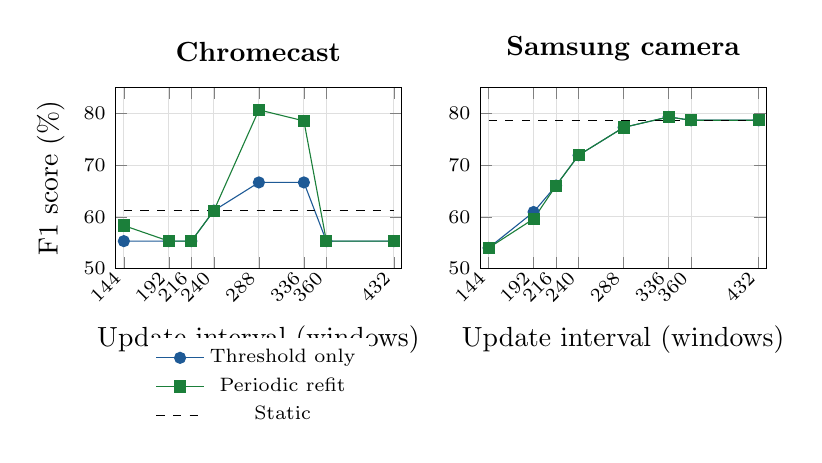
\begin{tikzpicture}
\begin{groupplot}[
  group style={group size=2 by 1, horizontal sep=1cm},
  width=0.43\textwidth,
  height=0.32\textwidth,
  xmin=135,
  xmax=440,
  ymin=50,
  ymax=85,
  xtick={144,192,216,240,288,336,360,432},
  x tick label style={font=\scriptsize,rotate=45,anchor=east},
  y tick label style={font=\scriptsize},
  grid=major,
  grid style={gray!25},
  xlabel={Update interval (windows)},
  ylabel={F1 score (\%)},
  title style={font=\bfseries},
  legend style={font=\scriptsize,draw=none,at={(0.5,-0.38)},anchor=north},
]
\nextgroupplot[title={Chromecast}]
\addplot[color=linkblue,mark=*] coordinates {
  (144,55.32) (192,55.32) (216,55.32) (240,61.22)
  (288,66.67) (336,66.67) (360,55.32) (432,55.32)
};
\addlegendentry{Threshold only}
\addplot[color=workinggreen,mark=square*] coordinates {
  (144,58.33) (192,55.32) (216,55.32) (240,61.22)
  (288,80.70) (336,78.57) (360,55.32) (432,55.32)
};
\addlegendentry{Periodic refit}
\addplot[color=black,dashed] coordinates {(144,61.22) (432,61.22)};
\addlegendentry{Static}

\nextgroupplot[title={Samsung camera},ylabel={}]
\addplot[color=linkblue,mark=*] coordinates {
  (144,54.00) (192,60.95) (216,66.06) (240,71.93)
  (288,77.31) (336,79.34) (360,78.69) (432,78.69)
};
\addplot[color=workinggreen,mark=square*] coordinates {
  (144,54.00) (192,59.62) (216,66.06) (240,71.93)
  (288,77.31) (336,79.34) (360,78.69) (432,78.69)
};
\addplot[color=black,dashed] coordinates {(144,78.69) (432,78.69)};
\end{groupplot}
\end{tikzpicture}
\caption{Exploratory development sensitivity to update cadence.}
\label{fig:cadence-sensitivity}
\end{figure}

With an update interval of 288 windows, Samsung does not perform the early update
that caused the loss at window 144, while Chromecast still refits once before
the later attacks. The selected configuration requires 240 accepted windows
because both devices had at least that many at the useful update. Figure
\ref{fig:cadence-sensitivity} also shows why this remains a development result:
the apparent best interval depends strongly on when attacks occur in these two
streams.

\subsection{Adaptation safety findings}

After each run, the labels were used to count how many attack windows had been
accepted into the adaptation buffer. The detector itself did not use those
labels when it selected windows or updated its state. This check shows that the
safety gate rejected all Chromecast attacks before the first update, but
accepted 22 Samsung attack windows.

\begin{table}[H]
\centering
\small
\begin{tabular}{llrrr}
\toprule
\textbf{Device} & \textbf{Update} & \textbf{Accepted windows} &
\textbf{Attack windows} & \textbf{Contamination} \\
\midrule
Chromecast & 288 & 285 & 0 & 0.00\% \\
Chromecast & 432 & 288 & 3 & 1.04\% \\
Samsung camera & 288 & 241 & 22 & 9.13\% \\
Samsung camera & 432 & 288 & 20 & 6.94\% \\
\bottomrule
\end{tabular}
\caption{Attack windows found in each periodic-refit buffer after the run.}
\label{tab:safe-contamination}
\end{table}

Increasing the score margin alone did not remove the Samsung contamination.
Those attacks already look ordinary to a detector that observes only four
protocol proportions. This supports an independent volume or rate safeguard
rather than a larger value of the same composition-score margin.

Refitting also changes the total concentration $\alpha_0$. The Chromecast value
moves moderately, whereas the Samsung value becomes more than nine times larger
under the selected configuration.

\begin{table}[H]
\centering
\small
\begin{tabularx}{\textwidth}{l>{\raggedright\arraybackslash}Xrrr}
\toprule
\textbf{Device} & \textbf{Experiment} & \textbf{Initial $\alpha_0$} &
\textbf{Final $\alpha_0$} & \textbf{Ratio} \\
\midrule
Chromecast & Periodic refit, 144/144 & 28.10 & 36.05 & 1.28 \\
Chromecast & Periodic refit, 288/240 (selected) & 28.10 & 34.47 & 1.23 \\
Samsung camera & Periodic refit, 144/144 & 17.39 & 206.40 & 11.87 \\
Samsung camera & Periodic refit, 288/240 (selected) & 17.39 & 166.62 & 9.58 \\
\bottomrule
\end{tabularx}
\caption{Movement of Dirichlet concentration during promoted refits. In each
periodic-refit name, the first number is the update interval and the second is
the minimum number of accepted windows required for refitting.}
\label{tab:alpha-movement}
\end{table}

Convergence and a better fit to the accepted buffer are therefore not enough to
make a refitted model safe. The next safeguard should limit how far the alpha
parameters can move, either by averaging the old and new values or by rejecting
an excessive change in total concentration.

\subsection{LM backend evidence}

Figure~\ref{fig:lm-runtime} compares LM and SciPy directly on the D-Link,
Chromecast, and Samsung training matrices. Both backends were run through the
same production code for each dataset on 9 September 2026. Model fitting is
shown in milliseconds; the two faster operations are shown in microseconds.

\begin{figure}[H]
\centering
\begin{tikzpicture}
\begin{groupplot}[
  group style={group size=3 by 1, horizontal sep=0.8cm},
  ybar,
  bar width=5pt,
  width=0.29\textwidth,
  height=0.31\textwidth,
  ymin=0,
  symbolic x coords={dlink,chromecast,samsung},
  xtick=data,
  xticklabels={D-Link,Chromecast,Samsung},
  x tick label style={font=\scriptsize,rotate=28,anchor=east},
  y tick label style={font=\scriptsize},
  grid=major,
  grid style={gray!20},
  enlarge x limits=0.22,
  title style={font=\small\bfseries},
  legend style={font=\small,draw=none,at={(1.72,-0.36)},anchor=north,
    legend columns=2},
]
\nextgroupplot[title={Complete model fit},ylabel={Time (ms)},ymax=285]
\addplot[fill=linkblue!70] coordinates {
  (dlink,191.04) (chromecast,254.17) (samsung,42.46)
};
\addlegendentry{LM}
\addplot[fill=workinggreen!70] coordinates {
  (dlink,180.59) (chromecast,194.40) (samsung,34.47)
};
\addlegendentry{SciPy}

\nextgroupplot[title={Training likelihood},ylabel={Time ($\mu$s)},ymax=95]
\addplot[fill=linkblue!70] coordinates {
  (dlink,55.02) (chromecast,84.69) (samsung,45.69)
};
\addplot[fill=workinggreen!70] coordinates {
  (dlink,49.79) (chromecast,52.12) (samsung,31.57)
};

\nextgroupplot[title={Single-window score},ylabel={Time ($\mu$s)},ymax=15]
\addplot[fill=linkblue!70] coordinates {
  (dlink,12.00) (chromecast,12.22) (samsung,12.18)
};
\addplot[fill=workinggreen!70] coordinates {
  (dlink,13.18) (chromecast,13.22) (samsung,13.20)
};
\end{groupplot}
\end{tikzpicture}
\caption{Median LM and SciPy runtimes for three production workloads. A complete
fit excludes data loading and file output; training likelihood is one call on
the complete fit matrix; single-window scoring uses one non-silent window. Lower
is better.}
\label{fig:lm-runtime}
\end{figure}

\begin{table}[H]
\centering
\small
\begin{tabular}{lr}
\toprule
\textbf{Agreement measure} & \textbf{Stored value} \\
\midrule
Maximum relative alpha difference & $3.86\times10^{-7}$ \\
Maximum absolute score difference & $1.09\times10^{-5}$ \\
Decision mismatches & 0 of 270 \\
Flags from each backend & 3 \\
\bottomrule
\end{tabular}
\caption{LM and SciPy agreement in the D-Link production benchmark.}
\label{tab:lm-agreement}
\end{table}

The native matrix optimisation removes repeated LM setup while preserving the
row-wise model. A separate experiment reproduces the aggregate calculation used
by the reference study.

\begin{table}[H]
\centering
\small
\begin{tabular}{lrrr}
\toprule
\textbf{Architecture} & \textbf{Paired fits converged} &
\textbf{Likelihood-time reduction} & \textbf{Wall-time reduction} \\
\midrule
Reference-paper aggregate & 79 of 84 & 12.2\% & 8.8\% \\
\bottomrule
\end{tabular}
\caption{LM timing result for the aggregate reference-paper experiment.}
\label{tab:professor-benchmark}
\end{table}

That result applies only to the aggregate calculation. In the production
benchmark, LM is slower for complete fitting and matrix likelihood on all three
datasets, but slightly faster for single-window scoring. The numerical agreement
in Table~\ref{tab:lm-agreement} shows that the backend choice does not change the
D-Link decisions.

\section{Temporal Evaluation Improvements}
\label{sec:temporal-wip}

\subsection{Why chronological capture splits were not enough}

The master split already moves forward in time and keeps each capture intact.
This is much safer than randomly mixing ten-minute windows, but it gives only one
answer for one choice of fitting, calibration, and development dates. Device
behaviour can change with its operating state, daily routine, or traffic volume,
so a detector that works after one boundary may perform differently when that
boundary moves by a day.

The windows are also not independent repetitions. A cloud upload, scanning
burst, or attack can continue across several consecutive windows. Autocorrelation
measures this relationship; at a lag of one it compares each ten-minute window
with the window immediately after it. Within individual captures, Chromecast
total packet counts had an autocorrelation of about $0.86$, while Samsung
protocol proportions ranged from about $0.46$ to $0.60$. The anomaly scores were
also correlated across adjacent windows, at about $0.39$ for Chromecast and
$0.42$ for Samsung. These values do not prove that the Dirichlet--multinomial
model is wrong, but they do show that 144 windows from one day are not equivalent
to 144 independent days of evidence.

For the same reason, six adjacent attack windows may represent one continuing
attack rather than six separate incidents. Window-level precision and recall
remain useful, but the evaluation must also group consecutive alerts and labels
into episodes. Episode recall answers whether an attack was detected at all;
false-alert episodes per day describe how often an operator would be interrupted;
and detection delay shows how long the detector took to react. Results should
also remain visible for each capture so one poor day cannot be hidden inside a
large pooled confusion matrix.

The improved architecture therefore keeps complete captures together and repeats
the evaluation at several points in time. Each fold uses earlier normal captures
to fit the model, later normal captures to calibrate its threshold, and a
still-later capture to measure performance. The fitting history expands in the
next fold, while the final-test captures remain untouched.

Before these folds are used to select final settings, the temporal branch must be
combined with the current detector. The master branch should check the actual
time ranges inside every capture and record how overlapping or complementary
fragments were handled. Each fold should keep its own model, threshold, events,
and report, and results should be shown by capture and attack episode. If the
thesis reports confidence intervals, it should resample complete captures rather
than individual windows.

One D-Link data issue also remains: the October 8 and 9 fitting captures overlap
and must be resolved before the final model is fitted.

\subsection{Changes implemented on the temporal branch}

The \texttt{feature/temporal-model} branch orders every processed window by its
actual UTC start and end time. It stops when two captures overlap unless the
configuration explains how to resolve them, and it checks that fitting,
calibration, development, and final data occur in that order. For the known
exceptions, it combines three complementary Chromecast fragments. The report
records each decision.

The branch also defines expanding three-block folds:

\begin{center}
earlier fit history $\longrightarrow$ later threshold calibration
$\longrightarrow$ still-later validation
\end{center}

Each fold writes its model, threshold, events, and report to separate paths.
Besides the usual totals for individual windows, its report shows results for
each capture, groups consecutive attack windows into episodes, counts false-alert
episodes per day, and measures detection delay. Detector settings can then be
compared under a maximum false-alert rate chosen before the experiment. Final
captures remain outside every fold.

\subsection{Results from the temporal folds}

\begin{table}[H]
\centering
\small
\begin{tabularx}{\textwidth}{>{\raggedright\arraybackslash}p{0.18\textwidth}
>{\raggedright\arraybackslash}p{0.13\textwidth} r r r X}
\toprule
\textbf{Dataset} & \textbf{Fold} & \textbf{Windows} & \textbf{Window FP}
& \textbf{Episode recall} & \textbf{False-alert episodes/day} \\
\midrule
Chromecast & Benign 1 & 288 & 12 & -- & 4.00 \\
Chromecast & Benign 2 & 288 & 2 & -- & 1.00 \\
Chromecast & Labelled 3 & 474 & 4 & 0.70 & 0.91 \\
Samsung camera & Benign 1 & 81 & 1 & -- & 1.78 \\
Samsung camera & Labelled 2 & 556 & 4 & 0.82 & 0.78 \\
\bottomrule
\end{tabularx}
\caption{Committed temporal-fold reports. Episode recall is undefined in folds
without attack episodes.}
\label{tab:temporal-folds}
\end{table}

The two benign Chromecast periods contain the same number of windows, yet the
one-percent threshold produces 12 false alerts in one and two in the other. The
future false-alert rate is therefore not fixed by the calibration quantile. In
the labelled periods, the detector finds seven of ten Chromecast attack episodes
and 23 of 28 Samsung episodes. These figures describe the temporal branch only;
they cannot be compared directly with the adaptive results because that branch
was created before adaptation was implemented.

\section{Additional Detector Experiments}
\label{sec:experiment-wip}

\subsection{Purpose and relation to the master branch}

These experiments began because the static four-category
Dirichlet--multinomial detector missed several labelled attack windows. One clear
example was a high-rate UDP flood: its protocol proportions still resembled
normal traffic even though the device was sending far more packets. The
composition score evaluates the relative mixture of TCP, UDP, SSDP, and ARP
within a window; it does not decide whether that window's total traffic volume is
normal. Other missed attacks changed byte volume, TCP connection attempts, ARP
activity, or traffic direction without always making the four-category mixture
unlikely. The Dirichlet--multinomial model was therefore retained as the
baseline, but it was no longer treated as a complete detector by itself.

The \texttt{feature/volume-anomaly} branch tests the smallest additional
measurements that address those misses. It checks packet count, byte count, TCP
SYN count, ARP count, and traffic direction against ranges learned from benign
calibration data. The branch diverged before the current master architecture and
uses different artefact and evaluation formats, so its results remain
experimental until the selected changes are ported and rerun on the reference
devices.

\subsection{How the detector changed}

Figure~\ref{fig:experiment-evolution} shows the Chromecast development progression.
Each accepted change addressed an observed failure rather than adding a general
machine-learning model.

\begin{figure}[H]
\centering
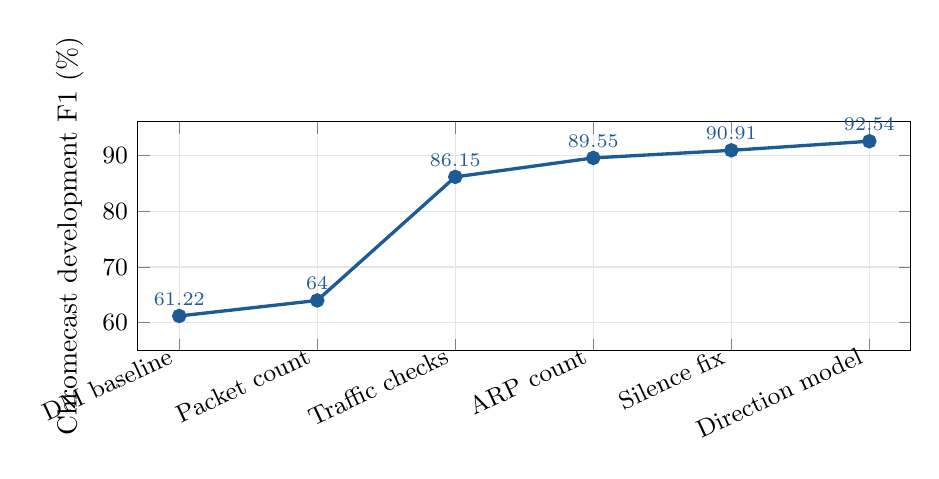
\begin{tikzpicture}
\begin{axis}[
  width=0.94\textwidth,
  height=0.37\textwidth,
  ymin=55,
  ymax=96,
  xmin=0.7,
  xmax=6.3,
  xtick={1,2,3,4,5,6},
  xticklabels={DM baseline,Packet count,Traffic checks,ARP count,Silence fix,Direction model},
  x tick label style={font=\small,rotate=25,anchor=east},
  y tick label style={font=\small},
  ylabel={Chromecast development F1 (\%)},
  grid=major,
  grid style={gray!20},
  mark options={solid},
  nodes near coords,
  nodes near coords style={font=\scriptsize},
]
\addplot[color=linkblue,very thick,mark=*] coordinates {
  (1,61.22) (2,64.00) (3,86.15) (4,89.55) (5,90.91) (6,92.54)
};
\end{axis}
\end{tikzpicture}
\caption{Changes that improved the experimental detector. Later score
normalisation changed the ranking of anomalies but did not change any alert.}
\label{fig:experiment-evolution}
\end{figure}

A high packet-count check detected one UDP flood without adding a false alert.
Separate checks for total bytes, TCP SYN packets, and traffic direction then
detected most of the remaining attack types. An ARP-count check detected the
low-rate ARP attacks. The next change stopped silent windows, which have no
traffic direction, from being flagged for that reason alone. Finally, a
two-category Dirichlet--multinomial model of incoming and outgoing traffic
replaced the raw incoming fraction. It reduced false alerts on later D-Link data
and detected one more Chromecast attack window.

The latest branch version puts the different feature scores on one scale. For
each feature, it records where a new score falls among that feature's benign
calibration scores. This change did not alter any development alert, but it made
the combined anomaly ranking easier to interpret. It also made the threshold
file larger because the benign calibration scores must be retained.

\subsection{Evidence across devices}

\begin{table}[H]
\centering
\small
\begin{tabular}{lrrrrrr}
\toprule
\textbf{Labelled development set} & \textbf{TP} & \textbf{TN} & \textbf{FP}
& \textbf{FN} & \textbf{F1} & \textbf{ROC--AUC} \\
\midrule
Chromecast & 31 & 438 & 4 & 1 & 92.54\% & 99.70\% \\
Amazon Echo & 9 & 458 & 5 & 3 & 69.23\% & 95.93\% \\
\bottomrule
\end{tabular}
\caption{Current development evidence on the experimental branch.}
\label{tab:experimental-labelled}
\end{table}

The completed detector was applied to Amazon Echo without retuning it for that
device. It detected every ARP attack window, but missed several low-rate UDP
windows because none of the added measurements was unusual enough. Compared
with protocol composition alone, it found one more attack window and incorrectly
flagged four more benign windows. This shows that the extra feature thresholds
still need cross-device calibration.

The branch also measures model size and scoring speed after score normalisation.

\begin{table}[H]
\centering
\small
\begin{tabular}{lrr}
\toprule
\textbf{Dataset} & \textbf{Model and threshold} &
\textbf{Mean latency per window} \\
\midrule
Chromecast & 99,957 bytes & 0.130 ms \\
Amazon Echo & 99,618 bytes & 0.077 ms \\
\bottomrule
\end{tabular}
\caption{Development-host edge-path measurements on the experimental branch.}
\label{tab:experimental-edge}
\end{table}

Python process memory, not detector state, dominates. These measurements support
gateway feasibility, but they do not replace testing on the intended edge
hardware.

\subsection{Final result from an earlier branch version}

Before later direction and fusion refinements, the six-feature Chromecast
architecture was frozen and evaluated once on its declared final partition.

\begin{table}[H]
\centering
\small
\begin{tabular}{lrrrrrrrr}
\toprule
\textbf{Partition} & \textbf{TP} & \textbf{TN} & \textbf{FP} & \textbf{FN}
& \textbf{Precision} & \textbf{Recall} & \textbf{F1} & \textbf{ROC--AUC} \\
\midrule
Chromecast final & 4 & 424 & 2 & 2 & 66.67\% & 66.67\% & 66.67\% & 99.77\% \\
\bottomrule
\end{tabular}
\caption{One-time final result for the earlier frozen experimental detector.}
\label{tab:experimental-final}
\end{table}

The 99.77\% ROC--AUC means that, when one attack window and one benign window are
compared, the detector almost always gives the attack window the more anomalous
score. This does not mean that every attack crosses the chosen alert threshold:
the fixed threshold detected four of the six attack windows and missed two.
Later branch iterations did not use this result for tuning. Even so, the labels
have now been examined, so this partition cannot be used to validate the later
direction model or score-ranking change. Those changes need another untouched
dataset or a new external test declared in advance.

The Echo final partition contained no labelled attacks and produced two alerts
in 432 windows. It supports normal-specificity evidence only; recall and F1 are
correctly undefined.

\subsection{Experiments that did not help}

Not every plausible feature improved the system. The branch deliberately removes
failed candidates while retaining their written reports.

\begin{table}[H]
\centering
\small
\begin{tabularx}{\textwidth}{>{\raggedright\arraybackslash}p{0.25\textwidth}
>{\raggedright\arraybackslash}p{0.18\textwidth} X}
\toprule
\textbf{Candidate} & \textbf{Decision} & \textbf{Reason} \\
\midrule
Adjacent-window byte change & Rejected & Recovered one Echo attack window but
added false alerts on both labelled devices and more D-Link alerts. \\
Mean packet-size tails & Rejected & Added many Echo false positives and did not
improve Chromecast attack recall. \\
Feature corroboration rules & Rejected & Suppressed valid single-signal attacks;
the only softer gain removed one shallow development false alert. \\
Automatic adaptive promotion & Rejected & A candidate that helped Chromecast
increased alerts on later unlabelled D-Link traffic, so the safety check rejected
it. \\
\bottomrule
\end{tabularx}
\caption{Experimental changes that were tested and rejected.}
\label{tab:rejected-experiments}
\end{table}

These failures are part of the project contribution. They show why more features
or more temporal state are not automatically better. The current experimental
endpoint keeps Minka fixed-point estimation, LM likelihood evaluation, and six
interpretable signals. It also requires a person to approve an adapted model
rather than promoting one automatically.

\subsection{Changes worth carrying forward}

The packet, byte, TCP SYN, and ARP counts are the clearest detector additions.
The direction model, results by attack episode, and detector-health report also
address observed failures and have evidence from more than one device. Score
normalisation is worth carrying forward only if the thesis needs one ranking or
severity scale across all features, because it substantially enlarges the
threshold file without changing the current alerts.

The rejected derivative, mean-size, corroboration, and automatic-promotion
variants should remain experiment records. They solve no demonstrated
cross-device problem. Any selected multi-signal subset must be ported into the
current master interfaces and rerun on both current master devices before it is
called part of the working system.

\section{What the Results Mean}

\subsection{Strengths demonstrated}

The project now demonstrates more than a statistical prototype. It provides a
complete evidence chain from source bytes and device identity to a model-bound
decision. The detector is unsupervised at fitting and adaptation time, results
are reproducible through named configurations, and the numerical backend has
been validated rather than merely selected.

The static results establish a high-precision baseline on two labelled devices,
but also show that four protocol proportions do not detect every attack. The
multi-signal experiments recover many of the missed attacks with simple,
interpretable measurements, while their rejected variants document where extra
features created more false alerts than useful detections. The temporal work
shows that performance changes across dates and must be reported by capture and
attack episode, not only as one pooled confusion matrix. The adaptation study
adds a separate lesson: periodic refitting can help, but only if the detector can
keep attack traffic out of the data used to update the model.

\subsection{Claims that remain too strong}

The current evidence does not justify calling \projectname{} a finished
edge-security product. Detection results come from two labelled devices and
mostly from one development split for each; window length has not yet been
compared, and no block-based confidence interval is available.

The adaptation configuration was tuned on the same development streams used to
report it, its Samsung buffer admits attack windows, and refitting can move the
model concentration too far. The temporal branch has not yet been combined with
the current detector, and the master detector has no locked final result. The
experimental Chromecast final run belongs to an earlier detector and cannot
validate later changes. Finally, the forecast command draws synthetic outcomes
from the model itself; it tests metric code, not forecasting accuracy on real
future traffic.

\section{Prioritised Completion Plan}

\subsection{First: validate the data splits}

The first merge should order data by actual timestamps, reject unexplained
overlaps, record how known capture fragments are handled, and report results by
capture and attack episode. The chronological folds must write to separate paths
so one run cannot overwrite another. These changes should be moved onto master
without changing the static detector.

\subsection{Second: compare detector versions}

The four-category system should remain the named static baseline. A separate
hybrid configuration can then add the smallest multi-signal subset supported by
the experiment branch. Packet volume is the most direct adaptation safeguard;
SYN, ARP, and direction evidence belong in the broader detection comparison.
Samsung must be included in the rerun because the experimental branch currently
contains Chromecast and Echo, not the complete reference pair.

This produces a clean scientific comparison: composition-only static, selected
hybrid static, adaptive threshold, and guarded periodic refitting. It avoids
quietly changing the baseline while the adaptation policy is being assessed.

The thesis will also include experiments on choices that currently remain fixed.
In particular, the complete pipeline will be rerun with window lengths such as
5, 10, 15, and 20 minutes on both labelled devices. The comparison will measure
whether shorter windows improve detection time enough to justify their sparser
counts, and whether longer windows improve model stability at the cost of slower
detection. Window length will be selected with the temporal development folds,
not with the final test data.

\subsection{Third: make adaptation safer}

The next adaptation experiment should change one safety mechanism at a time.
First, calculate a new threshold only from windows accepted by the safety gate,
and compare that result with periodic refitting that leaves the threshold fixed.
Next, limit how far a refit can move the alpha parameters by averaging the old
and new values or rejecting an excessive concentration change. Finally, check
that traffic volume is also normal before a window enters the refit buffer.

The temporal folds should be used for selection, with promotion judged on data
the candidate did not fit. Every chosen limit must have an operational
interpretation and be selected across devices rather than from the best point on
one curve.

\subsection{Fourth: freeze the system and run the final test}

After the architecture, thresholds, adaptation controls, code revision, dataset
fingerprint, and evaluation rule are frozen, the system needs one genuinely
untouched test. The master final partitions are still untouched by the master
pipeline, but the Chromecast dates have been opened in the experimental branch.
For a refined system, the strongest option is a new labelled device or external
dataset whose labels were not used during development.

Final reporting should include window and episode metrics, per-capture variation,
false-alert episodes per day, detection delay, and block-level uncertainty. Only
after this result should the selected detector be benchmarked on the intended
edge hardware. Empirical forecasting should either be implemented on held-out
traffic or removed from the thesis claims.

\section{Concluding Position}

\projectname{} is now a working research system rather than a collection of
separate scripts. On the master branch it validates packet captures, builds
device-specific count windows, fits and calibrates a Dirichlet--multinomial
model, scores later traffic, explains alerts, and evaluates labelled development
data. The native LM likelihood agrees closely with SciPy, and the stored metadata
make each result traceable to its data, model, and threshold. The static detector
is precise but misses attacks that do not change protocol composition enough.

The additional branches address two different limitations. The temporal branch
checks the real ordering of the data and reports performance by capture and
attack episode. The multi-signal branch tests simple measurements for traffic
volume, connection behaviour, ARP activity, and direction, and records both
successful and failed experiments. The 288/240 periodic-refit configuration is
also a useful adaptation candidate, but its Samsung buffer contamination and
large concentration change show why it is not yet a final choice.

The project is therefore ready to combine the proven data checks and detector
changes, compare window lengths and detector versions, and freeze a final
experimental protocol. Its main contribution so far is a transparent chain from
raw data to reproducible results, including evidence about what improved the
detector and what did not. A final thesis claim should follow only after the
combined system has been evaluated on untouched data.

\appendix

\section{Reproduction Commands}

The supported container runner is used from the repository root:

\begin{verbatim}
./scripts/run.sh preprocess --config configs/unsw_chromecast.json
./scripts/run.sh diagnose --config configs/unsw_chromecast.json
./scripts/run.sh train --config configs/unsw_chromecast.json
./scripts/run.sh calibrate --config configs/unsw_chromecast.json
./scripts/run.sh score --config configs/unsw_chromecast.json
./scripts/run.sh evaluate --config configs/unsw_chromecast.json
\end{verbatim}

The three paired timing runs in Figure~\ref{fig:lm-runtime} use:

\begin{verbatim}
./scripts/run.sh benchmark --config configs/d_link_day_cam5.json
./scripts/run.sh benchmark --config configs/unsw_chromecast.json
./scripts/run.sh benchmark --config configs/unsw_samsung_camera.json
\end{verbatim}

The complete stored adaptation comparison for both labelled devices is:

\begin{verbatim}
./scripts/run_adaptation_experiments.sh
\end{verbatim}

The script resolves the repository root itself, so the same command works when
invoked by absolute path or from another current directory. One selected adaptive
run can be reproduced with:

\begin{verbatim}
./scripts/run.sh adapt --config \
  configs/experiments/unsw_chromecast_periodic_refit_288_240.json
./scripts/run.sh evaluate --config \
  configs/experiments/unsw_chromecast_periodic_refit_288_240.json
\end{verbatim}

The Samsung command uses the corresponding Samsung configuration. On the
temporal branch, one fold is run with:

\begin{verbatim}
scripts/run_temporal_fold.sh \
  configs/temporal_folds/unsw_chromecast_fold_1.json
\end{verbatim}

\section{Repository Evidence Map}

\begin{longtable}{>{\raggedright\arraybackslash}p{0.34\textwidth}
>{\raggedright\arraybackslash}p{0.58\textwidth}}
\caption{Primary records supporting this report.}\label{tab:evidence-map}\\
\toprule
\textbf{Record} & \textbf{Evidence} \\
\midrule
\endfirsthead
\toprule
\textbf{Record} & \textbf{Evidence} \\
\midrule
\endhead
\path{docs/thesis_proposal_and_system_architecture.tex} & Original motivation,
research questions, theoretical basis, and intended architecture. \\
\path{docs/lm_idnet_project_status_report.tex} & Pre-adaptation reference-system
architecture and implementation record. \\
\path{docs/lm_idnet_adaptation_stage_report.tex} & Complete adaptation design,
experiments, contamination analysis, parameter sweep, and next controls. \\
\path{docs/lm_backend_change_record.tex} & Native changes relative to the
preserved professor-supplied source. \\
\path{docs/lm_professor_architecture_experiment_report.md} & Aggregate
reference-paper benchmark and comparison with the row-wise production detector. \\
\path{reports/D-LinkDayCam5/lm_backend_benchmark.json} & Production LM/SciPy
timing and numerical agreement. \\
\path{reports/UNSW-Chromecast/evaluation_statistics.json} & Static Chromecast
development confusion matrix and metrics. \\
\path{reports/UNSW-Samsung-Camera/evaluation_statistics.json} & Static Samsung
development confusion matrix and metrics. \\
\path{reports/experiments/} & Threshold-only and periodic-refit adaptation
audits, evaluations, and selected 288/240 evidence. \\
\path{docs/temporal_dataset_architecture_review_and_improvement.tex} & Temporal
dependence review and architecture rationale. \\
\texttt{feature/temporal-model} & Canonical timeline, expanding folds,
per-capture and episode metrics, and stored fold reports. \\
\texttt{feature/volume-anomaly} & Multi-signal experiments, third-device test,
locked branch result, edge measurements, and negative experiment records. \\
\bottomrule
\end{longtable}

\section{Selected Master Adaptation Configuration}

\begin{verbatim}
"adaptation": {
  "mode": "periodic_refit",
  "buffer_size": 288,
  "update_every": 288,
  "minimum_refit_windows": 240,
  "safe_margin": 1.0
}
\end{verbatim}

With ten-minute windows, 288 usable observations represent a nominal two-day
cadence. Missing windows are skipped, so elapsed wall-clock time can be longer.

\begin{thebibliography}{9}

\bibitem{iotpaper}
S. Al-Haj Baddar, A. Languasco, and M. Migliardi,
``Modeling and forecasting overdispersed IoT data using an efficient and accurate
computation of the Dirichlet Multinomial distribution,'' reference manuscript
supplied with the repository.

\bibitem{lmcore}
A. Languasco and M. Migliardi,
``On the fast computation of the Dirichlet-multinomial log-likelihood function,''
\emph{Computational Statistics}, vol. 38, pp. 1995--2013, 2023.
doi: \href{https://doi.org/10.1007/s00180-022-01311-7}{10.1007/s00180-022-01311-7}.

\bibitem{tpami}
S. Al-Haj Baddar, A. Languasco, and M. Migliardi,
``Efficient Analysis of Overdispersed Data Using an Accurate Computation of the
Dirichlet Multinomial Distribution,''
\emph{IEEE Transactions on Pattern Analysis and Machine Intelligence}, vol. 47,
no. 2, 2025.
doi: \href{https://doi.org/10.1109/TPAMI.2024.3489645}{10.1109/TPAMI.2024.3489645}.

\bibitem{minka}
T. P. Minka,
``Estimating a Dirichlet distribution,'' technical report, 2000; revised 2012.

\bibitem{yushaw}
P. Yu and C. A. Shaw,
``An efficient algorithm for accurate computation of the Dirichlet-multinomial
log-likelihood function,'' \emph{Bioinformatics}, vol. 30, no. 11,
pp. 1547--1554, 2014.
doi: \href{https://doi.org/10.1093/bioinformatics/btu079}{10.1093/bioinformatics/btu079}.

\end{thebibliography}

\end{document}
